% Gemini theme
% See: https://rev.cs.uchicago.edu/k4rtik/gemini-uccs
% A fork of https://github.com/anishathalye/gemini

\documentclass[final]{beamer}

% ====================
% Packages
% ====================

\usepackage[T1]{fontenc}
\usepackage{lmodern}
\usepackage[size=custom,width=120,height=72,scale=1.0]{beamerposter}
\usetheme{gemini}
% \usecolortheme{uchicago}
\usecolortheme{stanford}
\usepackage{graphicx}
\usepackage{booktabs}
\usepackage{tikz}
\usepackage{pgfplots}
\usepackage{subfig}
\usepackage{amsmath}
\usepackage{booktabs}
\usepackage{multirow}
\usepackage{float}
\pgfplotsset{compat=1.17}

% ====================
% Lengths
% ====================

% If you have N columns, choose \sepwidth and \colwidth such that
% (N+1)*\sepwidth + N*\colwidth = \paperwidth
\newlength{\sepwidth}
\newlength{\colwidth}
\setlength{\sepwidth}{0.025\paperwidth}
\setlength{\colwidth}{0.3\paperwidth}

\newcommand{\separatorcolumn}{\begin{column}{\sepwidth}\end{column}}


\title{Enhancing Game Control Through Hybrid Reinforcement Learning}


\author{Danhua Yan}

\institute[shortinst]{Department of Computer Science, Stanford University}

% ====================
% Footer (optional)
% ====================

\footercontent{
  % \href{rylanschaeffer.github.io}{rylanschaeffer.github.io} \hfill
  Stanford CS234 Default Project - Winter 2025 \hfill
  \href{mailto:dhyan@stanford.edu}{dhyan@stanford.edu}}
% (can be left out to remove footer)

% ====================
% Logo (optional)
% ====================

% use this to include logos on the left and/or right side of the header:
% \logoright{\includegraphics[height=7cm]{logos/cs-logo-maroon.png}}
% \logoleft{\includegraphics[height=7cm]{logos/cs-logo-maroon.png}}

% ====================
% Body
% ====================

\begin{document}

% This adds the Logos on the top left and top right
\addtobeamertemplate{headline}{}
{
    \begin{tikzpicture}[remember picture,overlay]
    %   \node [anchor=north west, inner sep=3cm] at ([xshift=0.0cm,yshift=1.0cm]current page.north west)
    %   {\includegraphics[height=5.0cm]{stanford_logos/Stanford-CS.png}}; % uc-logo-white.eps
      \node [anchor=north east, inner sep=3cm] at ([xshift=0.0cm,yshift=2.5cm]current page.north east)
      {
\includegraphics[height=7.0cm]{stanford_logos/Block_S_2_color.png}};
    \end{tikzpicture}
}

\begin{frame}[t]
\begin{columns}[t]
\separatorcolumn

\begin{column}{\colwidth}

  \begin{block}{Introduction}
    \begin{itemize}
        \item \textbf{Objective} what are you trying to solve? Reference current challenges and why your work is meaningful.
        \item \textbf{Motivation} what are you trying to solve? Reference current challenges and why your work is meaningful.
    \end{itemize}
  \end{block}

  \begin{block}{Background}
  problem setup + notation; maybe previous work
    % \begin{itemize}
    %   \item \textbf{BERT Model} Developed by Devlin et al., utilizes transformer architecture for contextual word relationships.
    %   \item \textbf{Consistency Learning} One of the key areas in SSL field, stands out for its proven effectiveness across numerous benchmarks.
    %   This approach ensures that a model produces consistent outputs for an unlabeled example, even when subjected to minor perturbations, such as the introduction of small noise.
    %   \item \textbf{Unsupervised Data Augmentation (UDA)} Proposed by Xie et al. \cite{xie2020unsupervised}, demonstrates that effective data augmentation of unsupervised
    %   label can significantly enhance the performance of supervised learning of NLP tasks on 
    %   limited labeled data.
    % \end{itemize}
  \end{block}
  
  \begin{block}{Methods}
      \begin{figure}[h]%
          \centering
          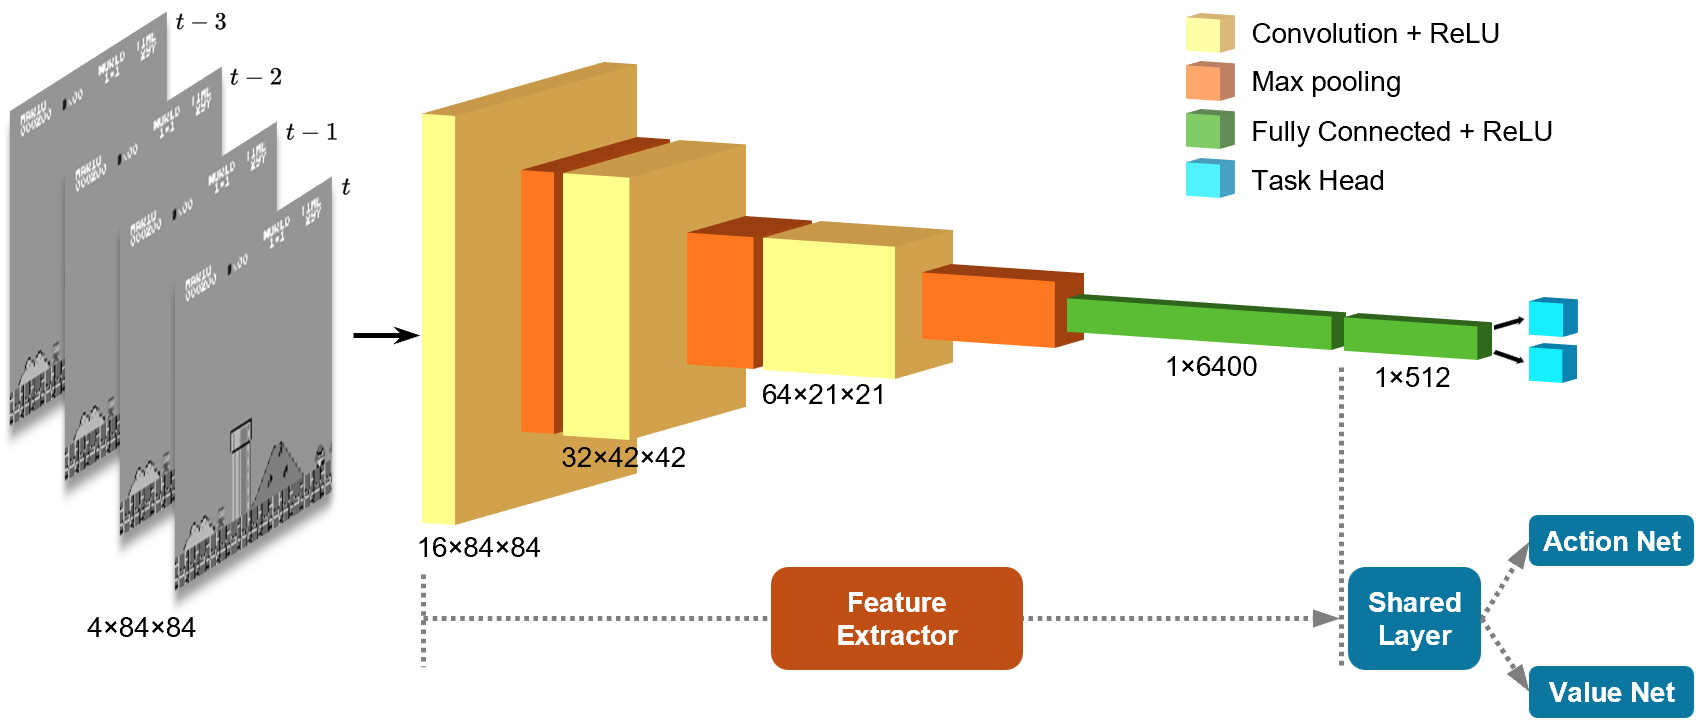
\includegraphics[width=0.9\textwidth]{pics/architecture.png}
          \caption{\textbf{PPO agent architecture for playing Super Mario Bros.}
            Four downsampled gameplay frames, ${f_{t-3}, \cdots, f_t}$, are stacked to represent the current state, $s_t$, preserving local temporal dynamics. The state $s_t$ is then processed through a three-layer CNN, producing a flattened dense feature representation. The actor-critic policy shares a common hidden layer, followed by separate action and value heads.
          }%
          \label{fig:example}%
      \end{figure}
    explain your technical contributions; figures can really help understanding especially for a neural model!
    % \textbf{Baseline} Uses frozen pre-trained BERT\textsubscript{BASE} embeddings with a single linear projection layer as task head.

    % \textbf{Combining Sentence Embeddings} (Figure \ref{fig:example})
    % \begin{itemize}
    %     \item {Pooling Separate Embeddings:} Generates a joint embedding from two sentences encoded separately by BERT.
    %     \item {Fused Sentence Embedding:} Utilizes BERT's inherent training 
    %     with sentence pairs separated by the \texttt{[SEP]} token to encode sentence context 
    %     similarities.
    % \end{itemize} 

    % \textbf{Training Strategies}
    % \begin{itemize}
    %     \item {Sequential Training:} Tasks are trained in succession 
    %     within each epoch. Specifically, model weights are updated per batch, with three tasks 
    %     forming a batch queue in the order of paraphrase detection, textual similarity, and 
    %     sentiment analysis.
    %     \item {Simultaneous Training:} Aggregates the losses for all tasks concurrently. 
    %     Each batch comprises three different tasks of the same batch size, and losses are 
    %     summed without weighting.
    % \end{itemize}
    
  \end{block}

  % \begin{alertblock}{A highlighted block}
  % \end{alertblock}

\end{column}

\separatorcolumn

\begin{column}{\colwidth}



  \begin{block}{Experiments}

        what is the task? What are the inputs and outputs to the model? What are the results? Compare against baselines; for results, a graph can say a lot more than a table of the same size!
  

    \textbf{Our highest performing model has test set overall accuracy of 0.763, 
    0.517 on SST5, 0.839 on QQP, and 0.866 on STS separately.}



    {\large
    \begin{table}[H]
      \centering
      \label{tab:baseline_ext}
      \begin{tabular}{@{}lcccc@{}}
        \toprule
        \textbf{Model} & \multicolumn{1}{c}{\textbf{SST5}} & \multicolumn{1}{c}{\textbf{QQP}} & \multicolumn{1}{c}{\textbf{STS}} & \multicolumn{1}{c}{\textbf{Acc}} \\ \midrule
        Baseline (last-layer only) & 0.309 & 0.667 & 0.209 & 0.527 \\
        Arc1-Simple Concat & 0.479 & 0.738 & 0.369 & 0.634 \\
        Arc1-Absolute difference & 0.510 & 0.733 & 0.532 & 0.670 \\
        Arc1-Dot Product Attention & 0.514 & 0.737 & 0.486 & 0.665 \\
        Arc2-Fused Sentence Embedding (BE) & 0.501 & 0.829 & 0.852 & 0.752 \\
        BE + Linear TSA & 0.520 & \textcolor{orange}{\textbf{0.836}} & 0.861 & \textcolor{orange}{\textbf{0.762}} \\
        BE + Linear TSA + UDA Back Translation & \textcolor{orange}{\textbf{0.520}} & 0.821 & \textcolor{orange}{\textbf{0.862}} & 0.758 \\
        BE + Linear TSA + UDA Sentence Completion & 0.506 & 0.820 & 0.853 & 0.751 \\
        BE + Linear TSA + UDA Random-mask Completion & 0.520 & 0.808 & 0.827 & 0.747 \\ 
        \bottomrule
      \end{tabular}
    \end{table}
    }
    


  \end{block}

\end{column}

\separatorcolumn

\begin{column}{\colwidth}

  \begin{block}{Analysis}
    \begin{figure}[H]%
      \centering
      \subfloat[SST5 Dev Set Confusion Matrix normalized to predicted labels]
      {{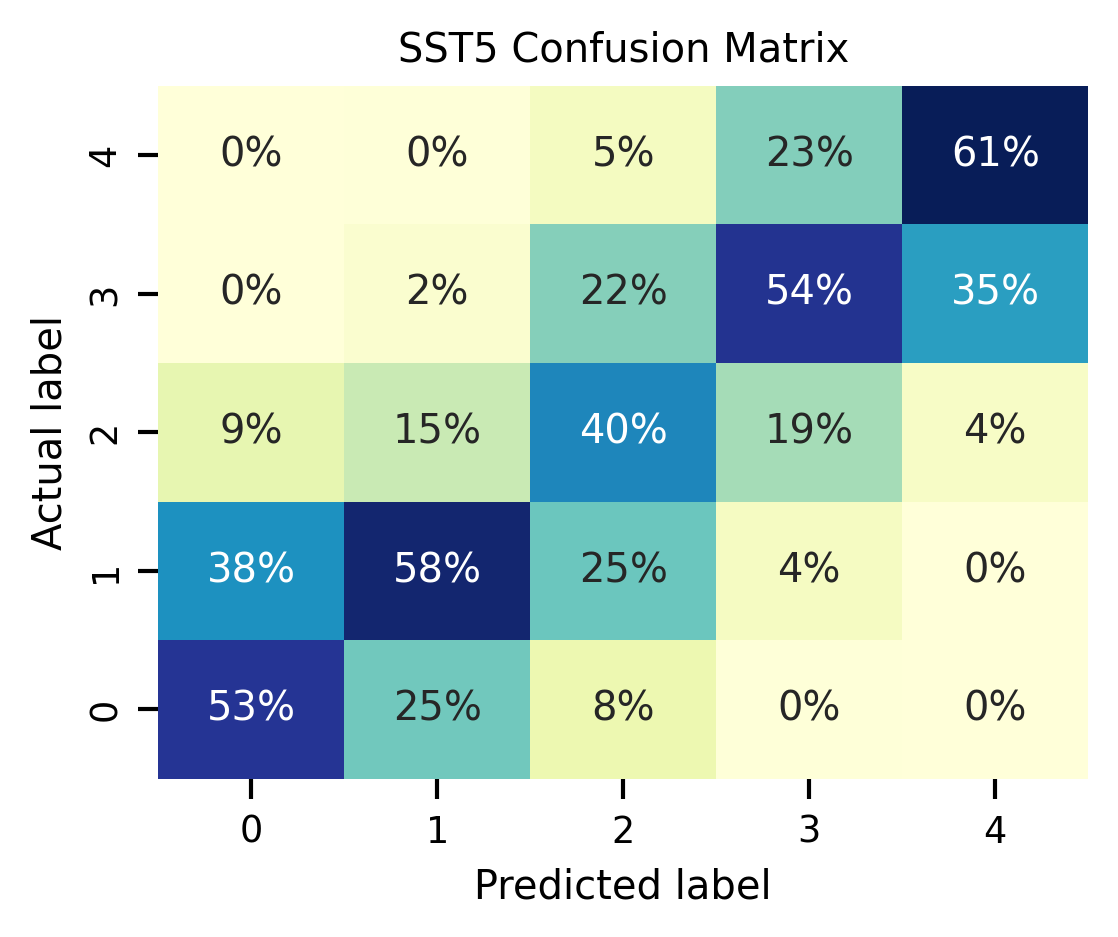
\includegraphics[width=0.3\textwidth]{pics/sst5.png} }}%
      \hfill
      \subfloat[QQP Dev Set Confusion Matrix normalized to predicted labels]
      {{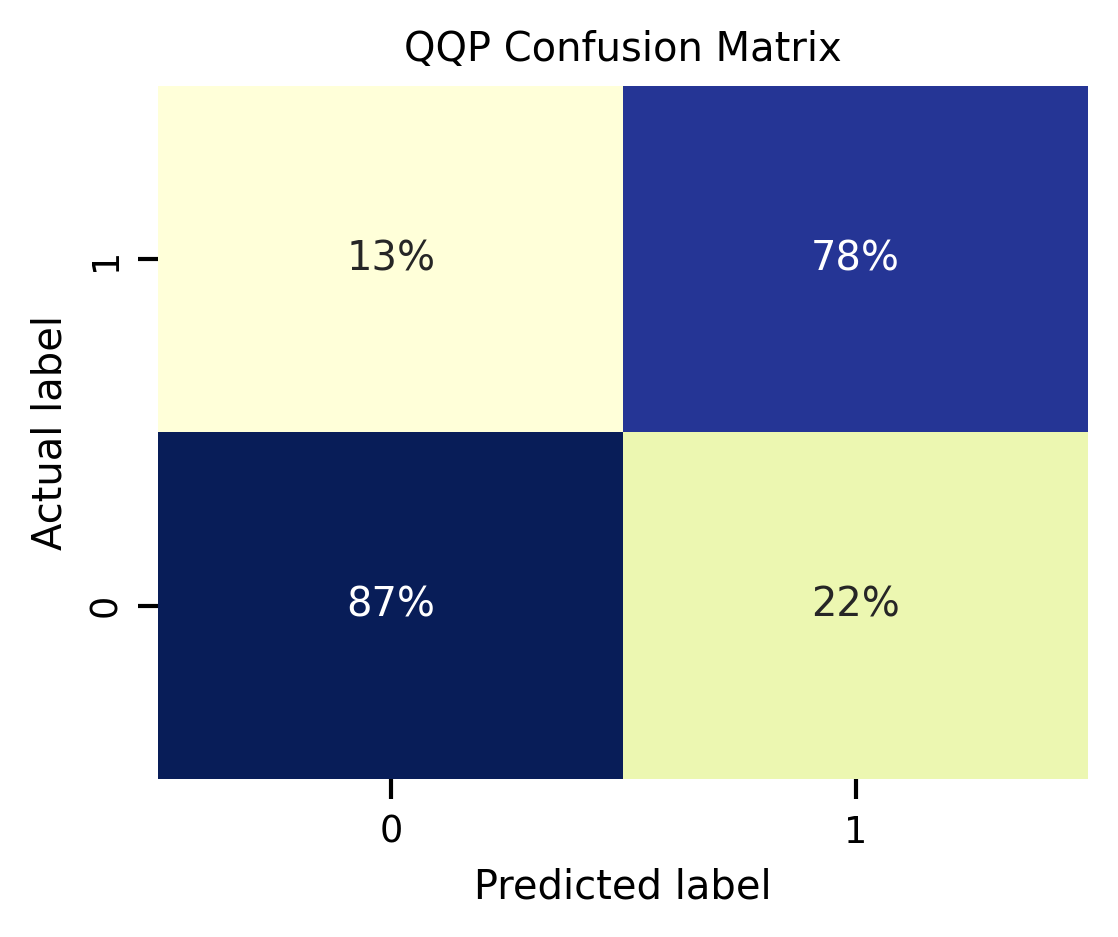
\includegraphics[width=0.3\textwidth]{pics/qqp.png} }}%
      \hfill
      \subfloat[STS Correlation Plot, line showing best fit]
      {{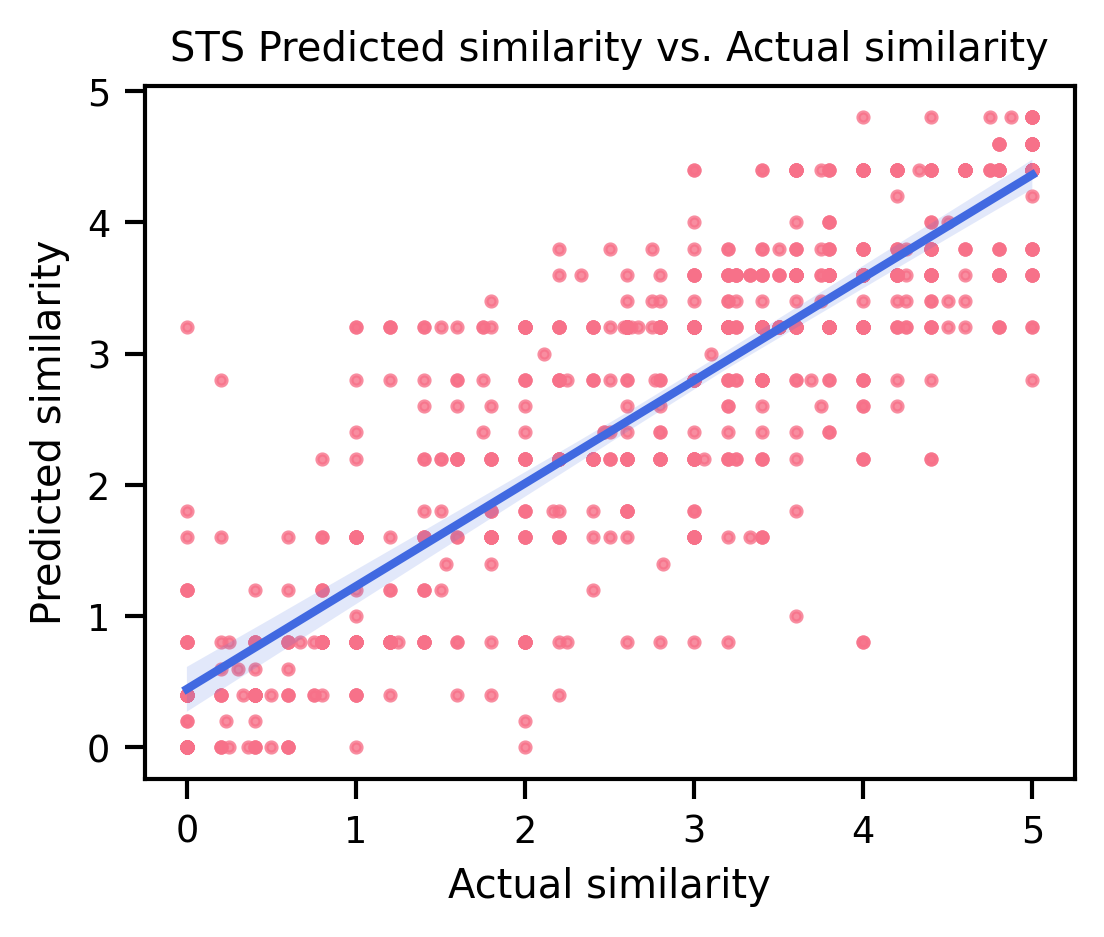
\includegraphics[width=0.3\textwidth]{pics/sts.png} }}%
      \caption{Analysis of Dev set performance of the model
      }%
      \label{fig:analysis}%
    \end{figure}
    provide some in-depth analysis of certain cases of interest, or contextualize your results within existing literature! Add some plots/examples/visualizations.
  \end{block}

  \begin{block}{Conclusion}
    briefly draw some conclusions from the work
    \cite{xie2020unsupervised}
  \end{block}

  % \begin{block}{References}
  % \noindent\rule{\textwidth}{1pt}
  \heading{Reference}
  \bibliographystyle{plain}
  \bibliography{poster}
    % \nocite{*}
    % \footnotesize{}

  % \end{block}

\end{column}

\separatorcolumn
\end{columns}
\end{frame}

\end{document}
